\documentclass[a4paper,12pt]{article}
\usepackage[backend=biber, citestyle=authoryear, bibencoding=utf8]{biblatex}
\addbibresource{./bibs/experimental-design.bib}
\addbibresource{./bibs/digital-ads.bib}
\addbibresource{./bibs/extra.bib}

\usepackage{amsmath, amsthm, amsfonts, mathtools, csquotes, bm, centernot, bbm, multirow, rotating, geometry}
\usepackage[toc,page]{appendix}
\usepackage{booktabs}
\usepackage[T1]{fontenc}

\geometry{a4paper, margin=2.5cm}

\title{Facebook Ads vs. Malaria: A Cluster-Randomized Trial in India}

\begin{document}
\maketitle

\begin{abstract}
We conduct a cluster-randomized trial on Facebook to measure the effectiveness of a social-media campaign on several self-reported outcomes of interest in the fight against malaria: preventative behaviors, treatment-seeking behaviors, and incidence of fever and malaria. We additionally nest an individually-randomized trial, utilizing the remarketing tools of the ad platform, to test the direct effect of advertising on individual behavior.

The novel study designs test full-scale, ``in the wild'' advertising campaigns run by and in collaboration with the organization Malaria No More. Outcomes are measured with survey responses and incentivized respondents recruited via a separate Facebook ad campaign, disconnecting the treatment and survey process and reducing response bias by design. To the best of our knowledge, this is the first research on social media campaigns for development outcomes to use such a design. The software used to optimize stratified recruitment and remarket to survey respondents is presented as an open source tool.

The results provide evidence of an increased use of mosquito nets due to treatment in certain subgroups. We also nest an individually-randomized trial into our design that shows evidence for an increase in preventative behavior for those individuals who were shown ads on their timelines, consistent across all studied subgroups. We conclude that ad campaigns can change behavior, but advanced targeting might be needed to reach subgroups of interest.



\end{abstract}

\clearpage

\section{Introduction}

A common concern about using social media campaigns for development outcomes is the lack of equity inherent in the audience. Social media reaches those who are connected to the internet, those who have smartphones, those who have money. The poorest and most at risk are thus potentially less effectively reached by interventions that rely on smart phones and internet connections when compared to richer, more urban populations.

Digital advertising, unlike traditional advertising media, provides the ability to microtarget messages to specific segments of the population, even if that segment is very small. This ability, however, is not all-powerful: certain segments of the population are easier to target than others and targeting might be difficult, requiring advanced knowledge and techniques.

Similarly, digital ad platforms provide a wealth of data on the reach and engagement of an ad campaign to evaluate its effectiveness, even allowing the user to segment such results by demographic characteristics. However, these segments may not be the segments of interest for the question at hand: age and gender might not predict malaria risk, while segments such as socioeconomic status are generally not available. Similarly, reach and engagement are not evenly distributed across the population, they are biased by the optimization routines, auction prices, sharing behavior, and time spent on social media.

Thus, digital advertising (and social media advertising in particular) present both a challenge and a potential solution: on the one hand, the audience is skewed away from populations of interest for development work, while on the other hand, the advertising can be intentially skewed to counter that effect.

We evaluate a Facebook ad campaign run by a public health non-profit (Malaria No More) with the help of a social media marketing consulting firm (Upswell) and funded by Facebook's Campaigns for a Healthier World initiative. We recruit a group of survey respondents and work directly with the advertising team to randomize application of the campaign by geography, dividing our respondents into control and treatment groups clustered at district level. We estimate the impacts of the campaign on a set of self-reported attitudes, behaviors, and medical outcomes as measured by the survey.

Malaria is a disease which disporportionately effects people in poor, rural areas in India (\cite{Dev2004}). In order to evaluate the impact of a social media campaign on malaria behaviors, attitudes, and incidence, it is therefore important to evaluate the impact specifically on populations that are at high risk for malaria. We analyze our initial baseline survey data to find predictors of malaria risk and find that dwelling type (i.e.\ concrete vs.\ mud/straw) is correlated with malaria incidence, in line with previous work in India (\cite{Sharma2015}).

We recruit survey respondents directly on Facebook via advertisements, where we offer mobile credit as an incentive to fill out survey. We find that in our initial recruitment, those living in permanent/concrete (pucca) dwellings make up the majority of respondents and those living in less-permanent/non-concrete (kutcha) dwellings were less likely to join our survey.

Facebook's ad targeting does not, out-of-the-box, allow us to target ads at those most at risk for malaria or those who live in kutcha dwellings. However, like many digital ad platforms, they do provide a set of tools to target ``people like those previous ones you sent me the other day.'' These are general-purpose marketing tools primarily used to find ``more good customers'' that hand-over the statistical problem of predicting outcomes from visible characteristics to Facebook's black box algorithms that have access to vast amounts of user data that can potentially be used in posed prediction problem.

In this study, we use their Lookalike Audience tool to target those living in kutcha dwellings and show that this technique works to increase the amount of non-pucca respondents we recruit to our surveys. We believe these techniques can, and should, be used to target public good campaigns at those most in need and we publish the software we created to do this as an open source platform called Virtual Lab. The platform allows users to recruit survey respondents and use them to create Lookalike Audiences that can be used to either recruit further respondents or for targeting in large-scale interventions.

By stratifying our recruitment by dwelling type, we were able to perform subgroup analysis and show that the main ad campaign increased the likelihood of sleeping under mosquito nets for those in pucca dwellings, but did not have a similar effect on those in other dwellings. There are two reasons this might be the case that we would like to split apart: A) the ad material itself had a greater effect on those who live in pucca dwellings and B) the ad campaign was mostly shown to those who live in pucca dwellings.

In order to differentiate the two hypotheses, we test the direct effect of the ad material on individuals by nesting an individually-randomized trial inside a second round of data collection. We use the remarketing tools of Facebook to directly target half of our survey respondents with ads, running a 2-week campaign in which we reached our target group with an average of 7 ads each. The ads show up on their timeline, like any ad, and respondents do not have any way of knowing that any particular ad came from us. After one week, we send them a follow-up survey asking if they slept under a mosquito net the previous night. We find that the ad campaign has a significant positive effect on people across all dwelling types.

We conclude that the ad material itself is effective at motivating people to take preventative action and use mosquito nets. The campaign itself was also effective at large scale for those it reached, but it may not have reached those most at risk. We therefore encourage the use of advanced targeting on digital ad platforms to ensure ads reach not only those who are the cheapest to advertise to, but also those who are most in need of the campaign.


\section{Background and Contribution}

\paragraph{Ad campaigns for public health outcomes in low- and middle-income countries.} There is some evidence that public health related ad campaigns in LMICs can shape opinions and behaviors in reproductive health (\cite{Agha2012}), attitudes towards smoking laws (\cite{Alday2010}), and preventative behaviors related to cancer screening (\cite{Wichachai2016}). However, the evidence is limited and to the best of our knowledge none evaluate social media campaigns (for a comprehensive review of social marketing studies in LMICs, see \cite{Schmidtke2021}).

Bannor et. al.\ conducted surveys of 150 members of the general public in Ghana and asked them questions about social media usage and health-related messages (\cite{Bannor2017}). Their findings emphasize the importance of social media as an avenue for communication: 79\% of respondents said they had recieved health-related messages on Facebook and 67\% reported that they took health-related messages found on social media seriously.

In high-income countries, digital and social media campaigns have been researched and shown effective in changing behavior in areas such as substance abuse (\cite{Evans2020}). Traditional media (television/print) campaigns have been tested in cluster-randomized trials and shown effective for public health outcomes such as the prevention of childhood obesity (\cite{Croker2012}).

% TODO: add something about malaria! Different interventions, impacts, etc.

This is the first study, to our knowledge, showing the effect of a digital ad campaign on malaria-related outcomes and provides substantive evidence that this messaging channel can be an important tool in fighting malaria and similar diseases by promoting preventative behavior.


\paragraph{Evaluating behavior change in social media social marketing campaigns}

Social marketing focuses on the use of marketing tools for behavioral change (\cite{Andreasen1994}). Despite this focus on behavior change, however, evaluating social media social marketing campaigns has been, to our knowledge entirely, restricted to evaluating engagement metrics (\cite{Shawky2019}) and very little has been done to run experiments on the impact of social media campaigns on behavioral change.

In order to understand this gap, it can help to understand how digital marketing tools work in general and why engagement has become the de facto standard. Ad platforms provide tools for measuring both ``on-platform'' results (users interact with your Facebook page) as well as ``off-platform'' results that take place on a platform or place controlled by the advertiser (i.e.\ their store or their website). Major advertising platforms, such as Facebook and Google, offer libraries that advertisers can add to their website (SDKs) that send events from their website back to the advertising platform. This allows the advertisers website to function as an extension of the ad platform, with all the data being consolidated inside the ad platform which then offers tools to analyze and run experiments.

By their nature, the data is thus restricted to users who engage with the properties of the advertiser in some fashion, either on or off-platform. This is useful for any enterprise in which engagement is the goal or a prerequisite to the goal. The exception that proves the rule for the tools offered directly on advertiser platforms are Brand Lift Studies. These studies allow advertisers to embed a short survey into the ad platform. The survey is shown both to those who have seen their ads and those who haven't and the difference reported. The format is restricted to a couple of questions, microdata is not provided for analysis, and it's made explicit that the entity asking question is the advertiser themselves. That being said, it is a powerful tool that can certainly be useful to researchers in this space.

In social marketing, the end goal is not necessarily to get people to engage with the advertising entity but, rather, to change their beliefs, attitudes, and behaviors in the real world. While engagement can be a means to this end, the end in itself (behavior change) needs to be evaluated as well.

%% TODO: these references are pretty random, find the best ones...
To get around the limitations in measurement provided by the ad platforms, many researchers perform ``lab'' experiments to test the effect of campaign content on attitudes of viewers. For example, respondents might be recruited to join a survey which they take on a survey platform, where they are shown content within the survey itself, as a proxy for seeing content on a social media timeline (\cite{Henry2020,Donati2020}). Similarly, public relations / market research companies offer a pool of paid respondents and a series of tools to show ads to these respondants (including in realistic settings) and ask them questions afterwards (\cite{Evans2021}) or to create a pool of general respondents for quasi-experimental designs (\cite{Sampogna2017}). While these examples show convincing results and have the advantage of full control and rich data about participant actions, they have the disadvantage of the intervention being delivered to users during their active and conscious participation in a study.

We contribute to this literature by offering a design for an individually-randomized study where the treatment is delivered to survey respondents via remarketing\footnote{Remarketing is a tool offered by the major ad platforms by which an ad campaign can be run to a group of individuals who have previously interacted with the advertiser in some way. With the current deprecation of 3rd-party cookies, this implies either that the individual has come directly from an ad to a platform run by the advertiser or that the individual has shared either personally identifying data or directly connected their account (i.e.\ their Facebook or Google account) with the advertiser.}. This implies that the ads show up in participants' real news feed, bidding in real ad auctions and mixed with other real ads, advertised by an entity that has no apparent connection to the surveying entity itself. To our knowledge, this is the first example of this design in the literature and we believe it can be useful. Additionally, we offer an open source software tool, Virtual Lab, which can be used to facilitate such a study design (\cite{Rao2020}).


% TODO: add description of virtual lab

% \section{Recruiting and Surveying on Facebook}

% We use an open-source platform, developed by the research team, called Virtual Lab to recruit respondents with Facebook advertising and interview them via chatbot on Facebook Messenger (\cite{Rao2020}).


\section{Cluster Level Study}

\cite{Hayes2017} lay out three main reasons for adopting a cluster-randomized design:

\begin{enumerate}
\item The intervention is, by its nature, applied to a group.
\item To avoid spillovers/contamination.
\item To capture population-level effects.
\end{enumerate}

\noindent We adopt a cluster-randomized design for all three reasons:

\paragraph{Population-level treatment.} The intervention of interest is itself a digital ad campaign run on a large population with a finite budget. Digital ad campaigns run on large populations inherently choose the recipient of each ad and this choice is often driven by budget considerations: advertisers maximize X subject to the budget constraint. X might be reach (more individuals seeing one ad) or it might be engagement (target individuals most likely to click or share) or it might be impressions (more ads shown overall, regardless of recipient). In the real world, many digital ad campaigns involve a mix of all those choices for different types of content: some meant to raise awareness and some meant to be shared or engaged with.


\paragraph{Spillovers.} In particular, there might be A) spillovers on a household or family level, as treated individuals encourage others in their family to take precautions against malaria exposure, B) spillovers along the social graph as facebook advertising, which are facebook posts, are shared by individuals who are exposed to them, thus exposing their Facebook friends as well, and C) spillovers related to the infectious disease itself, malaria, where the reduction of malaria incidence among treated individuals could lead to the reduction of malaria incidence among people living nearby.

\paragraph{Population-level effects.} Related to the spillovers of the infectious disease itself, we're interested not just on the effects of the ad campaign on the direct reduction of one individual's risk, but on the population-level effect of mass behavior change on the individual risk of an average member from the population.


\subsection{Procedure}

Four states were set aside from the main campaign for impact evaluation: Uttar Pradesh, Odisha, Jharkhand, and Chhattisgarh. We removed capital districts entirely from the study, leaving us with 152 districts in the four states. Out of those districts, our goal was to select 80 for the study and recruit 20,000 people across those 80 districts, with 250 people per district. The 80 districts were selected for convenience: they would be the 80 districts in which it is cheapest to recruit participants on Facebook. Cost of recruitment on Facebook is driven  by many factors, but at the extreme it is primarily driven by lack of active population. It's important to note that this is, of course, a limitation: our study population does not reflect the entire state, it excludes some of the lesser connected and less populous districts.

% That being said, there is still substantial variety both across and within districts. See ??? for descriptive statistics.

%% TODO: add district-level descriptives

%% TODO add N number of districts
The selected districts were chosen by beginning recruitment in all districts and progressively dropping the more expensive ones. Additionally, the initial data served to allow us to understand malaria incidence and identify characteristics of individuals at risk. Some interesting things popped out of this initial analysis:

%% TODO: add N=?? to the 0 incidences of malaria
\paragraph{Odisha, with historically high malaria incidence, had very low incidence compared with the other states.} Inline with recent govermental data, we found that answers the question \textit{Have you, someone in your house, or any of your neighbors had malaria in the past 5 years?} were significantly less positive in Odisha, where only 6.7\% of respondenses were positive, as opposed to 19.4\%, 16.5\%, and 23.0\% in the other states. Additionally, in 11 out of 23 districts in Odisha, we found 0 incidents of malaria, and in only 5 districts was 5-year incidence above 10\%. Seeing these numbers, we decided to drop Odisha entirely from the study and choose our 80 districts from among the other states and their 123 districts.

\paragraph{Historical malaria incidence is correlated with current incidence, but not perfectly.} We asked both whether respondents or anyone in their household had had malaria in the last 5 years as well as whether they had had malaria in the last 2 weeks. While historical incidence was correlated with current incidence (Pearson's $\rho = 0.12$ on individual level and $\rho = 0.50$ when comparing districts by their average), one might have expected this correlation to be higher. Malaria definitely moves and having up-to-date information is clearly important on targeting efforts.



\paragraph{Dwelling type is the strongest individual predictor of current malaria incidence.} Respondents were asked which kind of house they live in: Kutcha (made of mud, tin, straw), Pucca (have cement/brick wall and floor), or Semi-pucca. This question showed the highest marginal correlation with 2-week malaria incidence ($\rho = -0.057$ coded as kutcha < semi-pucca < pucca) of any of the individual questions we asked (see Table \ref{tbl:baseline-corr}). Running a simple regression tree to find  good predictors of malaria incidence (figure \ref{fig:regression-tree}), we see that dwelling type is the most consistent predictor. It's correlated with education, distance from the nearest medical center, being unemployed, and caste. Dwelling type thus captures both poverty and rurality, as well as itself being a risk factor for malaria.


% Table created by stargazer v.5.2.2 by Marek Hlavac, Harvard University. E-mail: hlavac at fas.harvard.edu
% Date and time: Sun, Jun 06, 2021 - 01:51:51 PM
\begin{table}[!htbp] \centering 
  \caption{Marginal Correlations at Baseline} 
  \label{tbl:baseline-corr} 
\begin{tabular}{@{\extracolsep{5pt}} ccc} 
\\[-1.8ex]\hline 
\hline \\[-1.8ex] 
 & Malaria - 2 weeks & Malaria - 5 years \\ 
\hline \\[-1.8ex] 
Distance to Medical Center &  .037 &  .055 \\ 
Backward Caste &  .022 &  .049 \\ 
Family Size &  .028 &  .032 \\ 
Air Conditioning &  .010 & -.021 \\ 
Education & -.026 &  .032 \\ 
Dwelling & -.041 & -.059 \\ 
\hline \\[-1.8ex] 
\end{tabular} 
\end{table} 





\subsection{Stratifying Recruitment}

Understanding measurable risk factors for malaria allows us to define at-risk subgroups and estimate conditional treatment effects for them. This is both useful for transportability and external validity, as well as for answering the previously posed question, \textit{do social media campaigns reach and have an effect on at-risk populations?}.

We decided to focus on dwelling type, given the fact that it was a promising correlate of malaria risk as well as a well-defined and easy-to-communicate population. In order to later estimate subgroup effects, however, we need to ensure sufficient respondents from each dwelling type. In our initial recruitment, however, people in ``kutcha'' dwellings were significantly less likely to be recruited into our survey than those with other dwelling types. In fact, the majority of respondents lived in pucca dwellings.

To recruit more of the underrepresented kutcha dwellers, we use Virtual Lab to create a lookalike audience in Facebook and dynamically increase spending to that audience in districts where kutcha dwellers are most underrepresented (in particular, those districts in which kutcha dwellers make up less than 30\% of respondents). Thus, we end up with 160 strata in total, 80 for the districts and 2 for the dwelling type (defined as kutcha and non-kutcha).

The effect of this stratification can be seen in figure \ref{fig:recruitment}. It is worth pointing out several effects of this intentional recruitment: A) the overall number of of kutcha dwellers increases, making dwelling-type more even and allowing us to better estimate effects by dwelling-type, B) the variance of dwelling-type by district decreases, orthogonalizing dwelling from district and allowing us to better estimate the effect of dwelling type by preventing that effect from being absorbed into district-level effects in a multi-level model.

Another effect of stratifying recruitment, both by district and dwelling type, is that it changes the population that any average effects in our analysis estimate. Without stratification, effect estimates are valid for ``the population most likely to respond to recruitment ads on Facebook.'' With stratification, we create a synthetic population on which we estimate average and conditional average effects. This synthetic population is not out-of-the-box representative of any actual population in the real world and average effect estimates on this population cannot be naively interpreted as representing the average effect on any real-world population. By orthogonalizing variables (for example dwelling type) by stratifying them equally, however, the data is better suited to both estimating conditional effects and transporting to populations where such quantities (i.e.\ the percentage of people living in different dwelling types) are known.


% TODO: Add randomization stuff!!!

% \subsection{Randomization}

% Districts were randomized via a matched pair design (\cite{ref}), where matching was performed based on the Mahalanobis distance across district level variables collected in the baseline survey: , , , , , .

% Pair assignment was rerandomized until balance across the measured variables was achieved.

% Balance stats here!!!


\subsection{Data}

Our cluster level study seeks to measure the effects of the real world ad campaign run by Malaria No More and Upswell. Respondents may or may not have been directly exposed to the advertising itself (we cannot directly measure this exposure on an individual level). Respondents in districts where advertisements were shown are considered ``treated'' and those in districts where advertisements were not shown are considered the ``control'' group. As such, we are measuring both the direct and indirect effects of the ad campaign at a ``group'' level, as reported by the individuals from the group who responded to our recruitment advertisements and joined our study.

The study is performed in two ``rounds.'' In round 1, respondents are recruited in July and August of 2020. In round 2, respondents are recruited between January and March of 2021. The anti-malaria ad campaign run by Malaria No More and Upswell (the treatment) was run between September of 2020 and January of 2021.

Round 1 respondents participate in a panel survey where they are invited to answer the same set of questions every 17 days between the time of recruitment until December 2020. These questions measure disease incidence (of malaria and fever), treatment seeking (in the case of disease), and preventative behaviors (\textit{did you sleep under a mosquito net last night?}). The number of ``waves'' answered by these respondents varies, depending on how quick they were to answer the invitation to take another survey, up to a maximum of 9 waves. The first wave (``baseline'') and last wave (``endline'') had additional questions. All respondents who at least completed the baseline, regardless of how many intermediate waves they completed, were invited to complete the endline survey on December 19the.

Round 2 respondents participate in a cross-sectional survey where they are asked about disease incidence and treatment seeking behaviors. A subset of this group became part of the ``individual level study'' (section \ref{individual-effect}) and were later asked about behaviors after being individually treated with ads via remarketing.


%%% DESCRIPTIVE???

% map plots of district-level variables and variation
% map of districts and assignments



\subsection{Results}

Malaria incidence and, relatedly, behavior, varies greatly by district, as shown previously in the descriptive statistics. Because our unit of randomization is also the district and our outcomes are binary, our workhorse model will be a binomial random effects model (\cite{Hayes2017}):

\begin{align*}
logit(\pi_{ih}) &= \alpha + \sum_j \beta_j x_{jih} + u_h \\
u_h &\sim \mathcal{N}(0, \sigma_B^2)
\end{align*}

Where $x_{jih}$ represent the value of covariate $j$ for individual $i$ in district $h$, where we include the district-level treatment indicator and, in some specifications, interactions and controls as covariates. This model allows each district ($h$) to have its own intercept ($u_h$) in addition to the common intercept ($\alpha$) under the assumption that the random intercepts follow a normal distribution with learned variance $\sigma_B$. As a robustness check, all models are additionally run with an alternative specification: OLS with cluster-robust standard errors, clustered at district level, and weighted by responses when the outcome is averaged over responses. The results are qualitatively similar, with point estimates from the OLS largely agreeing with calculated odds ratios from the binomial model and standard errors comparable.

% TODO discuss OLS results
% A comparison and discussion is provided in appendix ???.

The data from the round 1 panel study is filtered to only contain answers after September 21st, approximately one month after the start of the advertising campaign. Only users who successfully completed at least 3 waves are considered.


\paragraph{Preventative behaviors: sleeping under mosquito nets.} Respondents were asked the following two questions every 17 days in the panel survey:

\begin{enumerate}
\item \textit{Did you sleep under a mosquito net last night?}
\item \textit{How many family members that live in your house (including yourself) slept under a mosquito net last night?}
\end{enumerate}

For the first question, results are analyzed assuming a binomial model where the number of trials is equal to the number of waves the respondent answered and the number of successes is equal to the number of times they answered yes to the question. The underlying assumption is that, asked at least 17 days apart, the answers are independent, conditional on the underlying latent probability of the individual to sleep under a bed net in any given night.

A similar model is used for the second question, but the interpretation is less straight forward. The percentage of household members who slept under a bednet is recorded each wave by taking the number reported and diving by the previously-reported total number of household members. That percentage is then averaged over the answered waves, and the resulting regression is weighted by the number of waves answered. This model can clearly be improved upon from a statistical perspective, but the results seem very robust to model choice: the OLS alternative, non-weighted by answered waves, returns qualitatively similar results.


Results are reported in table \ref{tbl:Sleeping Under Bednet - Panel}. A few notes: those in better dwellings (pucca and semi-pucca) generally sleep under mosquito nets significantly less than those in kutcha dwellings. Additionally, there is a significant positive effect of treatment for sleeping under mosquito nets on those in pucca dwellings, both individually (marginally from 61.1\% in the control to 65.0\% in the treatment group) and, even stronger, on the entire family (marginally from 61.2\% in the control to 67.6\% in the treatment group).



% Table created by stargazer v.5.2.2 by Marek Hlavac, Harvard University. E-mail: hlavac at fas.harvard.edu
% Date and time: Sun, Dec 19, 2021 - 07:27:27 PM
\begin{table}[!htbp] \centering 
  \caption{Sleeping Under Bednet - Panel} 
  \label{tbl:Sleeping Under Bednet - Panel} 
\begin{tabular}{@{\extracolsep{5pt}}lcccccc} 
\\[-1.8ex]\hline 
\hline \\[-1.8ex] 
 & \multicolumn{3}{c}{Self} & \multicolumn{3}{c}{Household} \\ 
\\[-1.8ex] & (1) & (2) & (3) & (4) & (5) & (6)\\ 
\hline \\[-1.8ex] 
 treatment & 0.06 & $-$0.04 & 0.17 & 0.08 & $-$0.12 & 0.30$^{**}$ \\ 
  & (0.09) & (0.10) & (0.14) & (0.09) & (0.11) & (0.12) \\ 
  & & & & & & \\ 
 pucca &  & $-$0.29$^{***}$ &  &  & $-$0.50$^{***}$ &  \\ 
  &  & (0.07) &  &  & (0.08) &  \\ 
  & & & & & & \\ 
 semipucca &  & $-$0.13$^{**}$ &  &  & $-$0.19$^{***}$ &  \\ 
  &  & (0.06) &  &  & (0.07) &  \\ 
  & & & & & & \\ 
 treatment:pucca &  & 0.21$^{**}$ &  &  & 0.38$^{***}$ &  \\ 
  &  & (0.09) &  &  & (0.09) &  \\ 
  & & & & & & \\ 
\hline \\[-1.8ex] 
Controls & No & Yes & No & No & Yes & No \\ 
Subgroup & All & All & Pucca & All & All & Pucca \\ 
Observations & 2,927 & 2,927 & 1,393 & 2,659 & 2,659 & 1,293 \\ 
\hline 
\hline \\[-1.8ex] 
\textit{Note:}  & \multicolumn{6}{r}{$^{*}$p$<$0.1; $^{**}$p$<$0.05; $^{***}$p$<$0.01} \\ 
\end{tabular} 
\end{table} 


\paragraph{Disease incidence: reported cases of malaria and fever.} Respondents were asked the follow questions, in round 1 (panel) and round 2 (cross section) respectively regarding fever:
\begin{enumerate}
\item \textit{Have you/someone in your family had a fever (100.4F / 38C or above) in the last two weeks?}
\item \textit{Have you/someone in your family had a fever (100.4F / 38C or above) since last August?}
\end{enumerate}

\noindent And the following two regarding malaria:
\begin{enumerate}
\item \textit{Have you/someone in your family had Malaria in the last two weeks?}
\item \textit{Have you/someone in your family had Malaria since last August?}
\end{enumerate}

In the round 1 panel data, we end up with counts for each time a person reports experiencing malaria in their family. One natural option for modeling such counts could be a Poisson process. When counted over participants, the malaria reports have a mean of 0.08 and a variance 0.12, so a Poisson model is not unrealistic. However, malaria reports within a family are, realistically, likely to be highly correlated even after 17 days, invalidating the primary assumption of independence of counts in a poisson process. We therefore perform our analysis as a binomial random effects regression on an indicator on whether or not respondents reported having malaria in at least one wave. Results are qualitatively identical to those of modeling the counts as a poisson process. We do the same with fever. Another advantage with modeling the binary occurence of disease here is that the procedure is identical for round 2 (cross section) data and the results more comparable.

Results are reported in table \ref{tbl:Malaria Incidence} and \ref{tbl:Fever Incidence} for malaria and fever respectively. We do not find evidence that the treatment had an impact on incidence of fever. However, in the round 2 data, malaria incidence is estimated to be lower among the treated pucca population. This is the same population that, according to our data, also increased their usage of bednets significantly due to the ad campaign. The subgroup estimates are not statistically significant, but the point estimate of the effect size would imply a marginal decrease in malaria incidence in this population from 4.6\% in the control to 3.7\% in the treated group, or an odds ratio of 0.81.

Recall that round 2 data was collected between January and March of 2021, while the ad campaign and round 1 data collection both ran between September and December of 2020. A decrease in malaria incidence in those who live in pucca dwellings could reasonably be expected as a lagged result driven by a positive behavioral change in mosquito net usage a few months earlier, as estimated in our panel data.



% Table created by stargazer v.5.2.2 by Marek Hlavac, Harvard University. E-mail: hlavac at fas.harvard.edu
% Date and time: Sat, Jun 05, 2021 - 03:50:35 PM
\begin{table}[!htbp] \centering 
  \caption{Malaria Incidence} 
  \label{tbl:Malaria Incidence} 
\begin{tabular}{@{\extracolsep{5pt}}lcccccc} 
\\[-1.8ex]\hline 
\hline \\[-1.8ex] 
 & \multicolumn{3}{c}{Round 1 Panel} & \multicolumn{3}{c}{Round 2 Cross Section} \\ 
\\[-1.8ex] & (1) & (2) & (3) & (4) & (5) & (6)\\ 
\hline \\[-1.8ex] 
 treatment & $-$0.11 & $-$0.28 & 0.14 & 0.11 & 0.27 & $-$0.22 \\ 
  & (0.18) & (0.24) & (0.30) & (0.17) & (0.19) & (0.24) \\ 
  & & & & & & \\ 
 pucca &  & $-$0.66$^{**}$ &  &  & $-$0.11 &  \\ 
  &  & (0.29) &  &  & (0.20) &  \\ 
  & & & & & & \\ 
 semipucca &  & $-$0.21 &  &  & $-$0.08 &  \\ 
  &  & (0.23) &  &  & (0.15) &  \\ 
  & & & & & & \\ 
 treatment:pucca &  & 0.41 &  &  & $-$0.50$^{*}$ &  \\ 
  &  & (0.36) &  &  & (0.26) &  \\ 
  & & & & & & \\ 
\hline \\[-1.8ex] 
Controls & No & Yes & No & No & Yes & No \\ 
Subgroup & All & All & Pucca & All & All & Pucca \\ 
Observations & 2,815 & 2,815 & 1,408 & 4,898 & 4,895 & 2,191 \\ 
\hline 
\hline \\[-1.8ex] 
\textit{Note:}  & \multicolumn{6}{r}{$^{*}$p$<$0.1; $^{**}$p$<$0.05; $^{***}$p$<$0.01} \\ 
\end{tabular} 
\end{table} 


\paragraph{Treatment seeking: seeking medical attention after fever.} Respondents who reported having experienced an instance of fever in their household were asked this follow up question: \textit{Did you seek medical help?}

We again use our binomial model, considering the number of trials to be the number of times they reported fever and the number of successes the number of times they reported having sought medical help. Round 2 (cross section) data is analyzed similarly, where each participant only has a single trial.

Results are reported in table \ref{tbl:Treatment Seeking}. In general, our data cannot say much about the impact on treatment seeking behaviors. This is partially due to the reduced sample size (not everyone had a fever!) and due to the fact that, in the cross-section where the sample size is a bit larger (N=1335), the vast majority report of participants who report having experienced fever ``since last August'' also report having sought medical treatment (95\% overall) with that tendency being even higher among the population who live in pucca dwellings. There is, however, suggestive evidence for a positive effect of the campaign on the treatment-seeking behavior of the non-pucca dwelling population, although the effects are not statistically significant, the effect size is consistent with an increase in likelihood to seek treatment from 84\% to 89\% in that population. This effect would be consistent with the suggestive evidence for a positive effect on malaria incidence in this population in round 2 (cross section) data as well, as higher treatment seeking would leads to higher reporting.



% Table created by stargazer v.5.2.2 by Marek Hlavac, Harvard University. E-mail: hlavac at fas.harvard.edu
% Date and time: Mon, Jun 07, 2021 - 06:21:28 PM
\begin{table}[!htbp] \centering 
  \caption{Treatment Seeking} 
  \label{tbl:Treatment Seeking} 
\begin{tabular}{@{\extracolsep{5pt}}lcccccc} 
\\[-1.8ex]\hline 
\hline \\[-1.8ex] 
 & \multicolumn{3}{c}{Round 1 Panel} & \multicolumn{3}{c}{Round 2 Cross Section} \\ 
\\[-1.8ex] & (1) & (2) & (3) & (4) & (5) & (6)\\ 
\hline \\[-1.8ex] 
 treatment & 0.23 & 0.43 & $-$0.13 & 0.42 & 0.49 & 0.34 \\ 
  & (0.22) & (0.29) & (0.30) & (0.32) & (0.39) & (0.52) \\ 
  & & & & & & \\ 
 pucca &  & 0.08 &  &  & 0.27 &  \\ 
  &  & (0.30) &  &  & (0.35) &  \\ 
  & & & & & & \\ 
 treatment:pucca &  & $-$0.51 &  &  & $-$0.14 &  \\ 
  &  & (0.41) &  &  & (0.54) &  \\ 
  & & & & & & \\ 
\hline \\[-1.8ex] 
Controls & No & Yes & No & No & Yes & No \\ 
Subgroup & All & All & Pucca & All & All & Pucca \\ 
Observations & 632 & 631 & 277 & 1,335 & 1,335 & 602 \\ 
\hline 
\hline \\[-1.8ex] 
\textit{Note:}  & \multicolumn{6}{r}{$^{*}$p$<$0.1; $^{**}$p$<$0.05; $^{***}$p$<$0.01} \\ 
\end{tabular} 
\end{table} 



\section{Individual Effect Study} \label{individual-effect}


\subsection{Procedure}

Within the round 2 (cross section) data collection, we embedded an additional individually-randomized study to test the effects of direct ad exposure on reported behavior and attitudes.

To facilitate this design, data for the cross-sectional study was collected in two phases. In the first phase, demographic questions, as well as questions about fever and malaria incidence were asked, but no questions were asked about behavior (sleeping under a net, etc.). The second phase was collect between 3-12 weeks after the first phase.

After the first phase, participants (N=4908) were randomized into treatment and control groups, with rerandomization being used to ensure balance across gender, caste, education, dwelling-type, as well as the treatment assignment of their district in round 1 of the study. The treatment group (N=2359) was then targeted via remarketing with ad campaign which was run, over the course of 2 weeks, exclusively targeting those individuals. 2,119 / 2359 were reached by at least one ad and participants in this group saw an average of 6.6 ads each over the course of 2 weeks.

10 days after the end of the ad campaign, the second phase of the survey was sent to the respondents via Facebook Messenger. We consider only those respondents who answered both waves (N=1791).

In the cluster-level study, our primary focus of stratification was geography and dwelling-type. Given that our primary questions of interest were at the household level, the demographic characteristics of the individual responding to the question was not the highest priority. In reality, this was a matter of budget constraints: stratifying is by its nature expensive and by stratifying so heavily by geography and dwelling, we were not able to stratify by any additional characteristics.

Because of those choices, the respondents we recruited for the cluster-level studies were heavily skewed in their demographics. For example, from all the respondents to our baseline survey in round 1 of data collection, 50\% were under 25 and 93\% were male. While we were mostly taking advantage of respondents from round 2 of the cluster-level study to create the individual study, we made an additional effort to recruit some additional respondents exclusively for the individual study, stratifying by age and gender to improve the balance slightly, ending up with only 39\% under 25 and 76\% male.


%% \subsection{Data}
%% descriptives?
%% show balance, describe randomization procedure

\subsection{Results}

The primary outcome of interest for this study was the answer to the question: \textit{Did you sleep under a mosquito net last night?}. Due to the design of the study, with respondents stratified by the treatment status of their district in the cluster-level study, we were able to estimate effects both from the previous district-level treatment and the direct effects of the new individual-level treatment.


\begin{align*}
  logit(\pi_{i}) &= \alpha + \sum_j \beta_j x_{ji}
\end{align*}

Where $x_{ji}$ represent the value of covariate $j$ for individual $i$ and we include the individual-level treatment indicator, the district-level treatment indicator from the cluster-level study, and, in some specifications, additional interactions and control variables. Results from the regression are shown in table \ref{tbl:Sleeping Under Bednet (Individual Level) - Logistic Regression}.

There is a significant positive effect of the individual level treatment on the probability that a respondent has slept under a mosquito net the previous night: the estimated marginal effect of treatment implies an increase in the probability of sleeping under a mosquito net from 69\% in the control group to 74\% in the treatment group. This effect maintains its effect size and statistical significance across all specifications. Especially interesting: the estimated effect size does not differ across dwelling type, unlike in the cluster-level treatment. The implication here is that, conditional on actually having the ads targeted to them, individuals across different dwelling types experience a similar increase in their tendency to sleep under a mosquito net on any given night.




% Table created by stargazer v.5.2.2 by Marek Hlavac, Harvard University. E-mail: hlavac at fas.harvard.edu
% Date and time: Thu, Oct 07, 2021 - 05:24:07 AM
\begin{table}[!htbp] \centering 
  \caption{} 
  \label{tbl:Sleeping Under Bednet (Individual Level) - Logistic Regression} 
\begin{tabular}{@{\extracolsep{5pt}}lcccccc} 
\\[-1.8ex]\hline 
\hline \\[-1.8ex] 
 & \multicolumn{6}{c}{Sleeping Under Bednet (Individual Level) - Logistic Regression} \\ 
\cline{2-7} 
\\[-1.8ex] & \multicolumn{6}{c}{Slept Under Net} \\ 
\\[-1.8ex] & (1) & (2) & (3) & (4) & (5) & (6)\\ 
\hline \\[-1.8ex] 
 treatment & 0.04 &  & 0.11 & 0.13 & 0.11 & 0.10 \\ 
  & (0.19) &  & (0.13) & (0.18) & (0.13) & (0.13) \\ 
  & & & & & & \\ 
 pucca & $-$0.66$^{***}$ &  & $-$0.60$^{***}$ &  & $-$0.61$^{***}$ &  \\ 
  & (0.23) &  & (0.20) &  & (0.23) &  \\ 
  & & & & & & \\ 
 semipucca & $-$0.16 &  & $-$0.16 &  & $-$0.16 &  \\ 
  & (0.20) &  & (0.20) &  & (0.20) &  \\ 
  & & & & & & \\ 
 admalaria &  &  &  &  &  & 0.69$^{***}$ \\ 
  &  &  &  &  &  & (0.17) \\ 
  & & & & & & \\ 
 ind\_treatment & 0.34$^{***}$ & 0.27$^{**}$ & 0.34$^{***}$ & 0.36$^{**}$ & 0.34$^{*}$ & 0.28$^{**}$ \\ 
  & (0.13) & (0.13) & (0.13) & (0.17) & (0.19) & (0.13) \\ 
  & & & & & & \\ 
 treatment:pucca & 0.12 &  &  &  &  &  \\ 
  & (0.26) &  &  &  &  &  \\ 
  & & & & & & \\ 
 ind\_treatment:treatment &  &  &  & $-$0.12 &  &  \\ 
  &  &  &  & (0.26) &  &  \\ 
  & & & & & & \\ 
 ind\_treatment:pucca &  &  &  &  & 0.01 &  \\ 
  &  &  &  &  & (0.26) &  \\ 
  & & & & & & \\ 
\hline \\[-1.8ex] 
Controls & Yes & No & Yes & Yes & Yes & Yes \\ 
Observations & 1,225 & 1,226 & 1,225 & 1,225 & 1,225 & 1,225 \\ 
\hline 
\hline \\[-1.8ex] 
\textit{Note:}  & \multicolumn{6}{r}{$^{*}$p$<$0.1; $^{**}$p$<$0.05; $^{***}$p$<$0.01} \\ 
\end{tabular} 
\end{table} 



\clearpage
\printbibliography

\clearpage
\appendix

\section{Figures}

\begin{figure}[h]
	\centering
	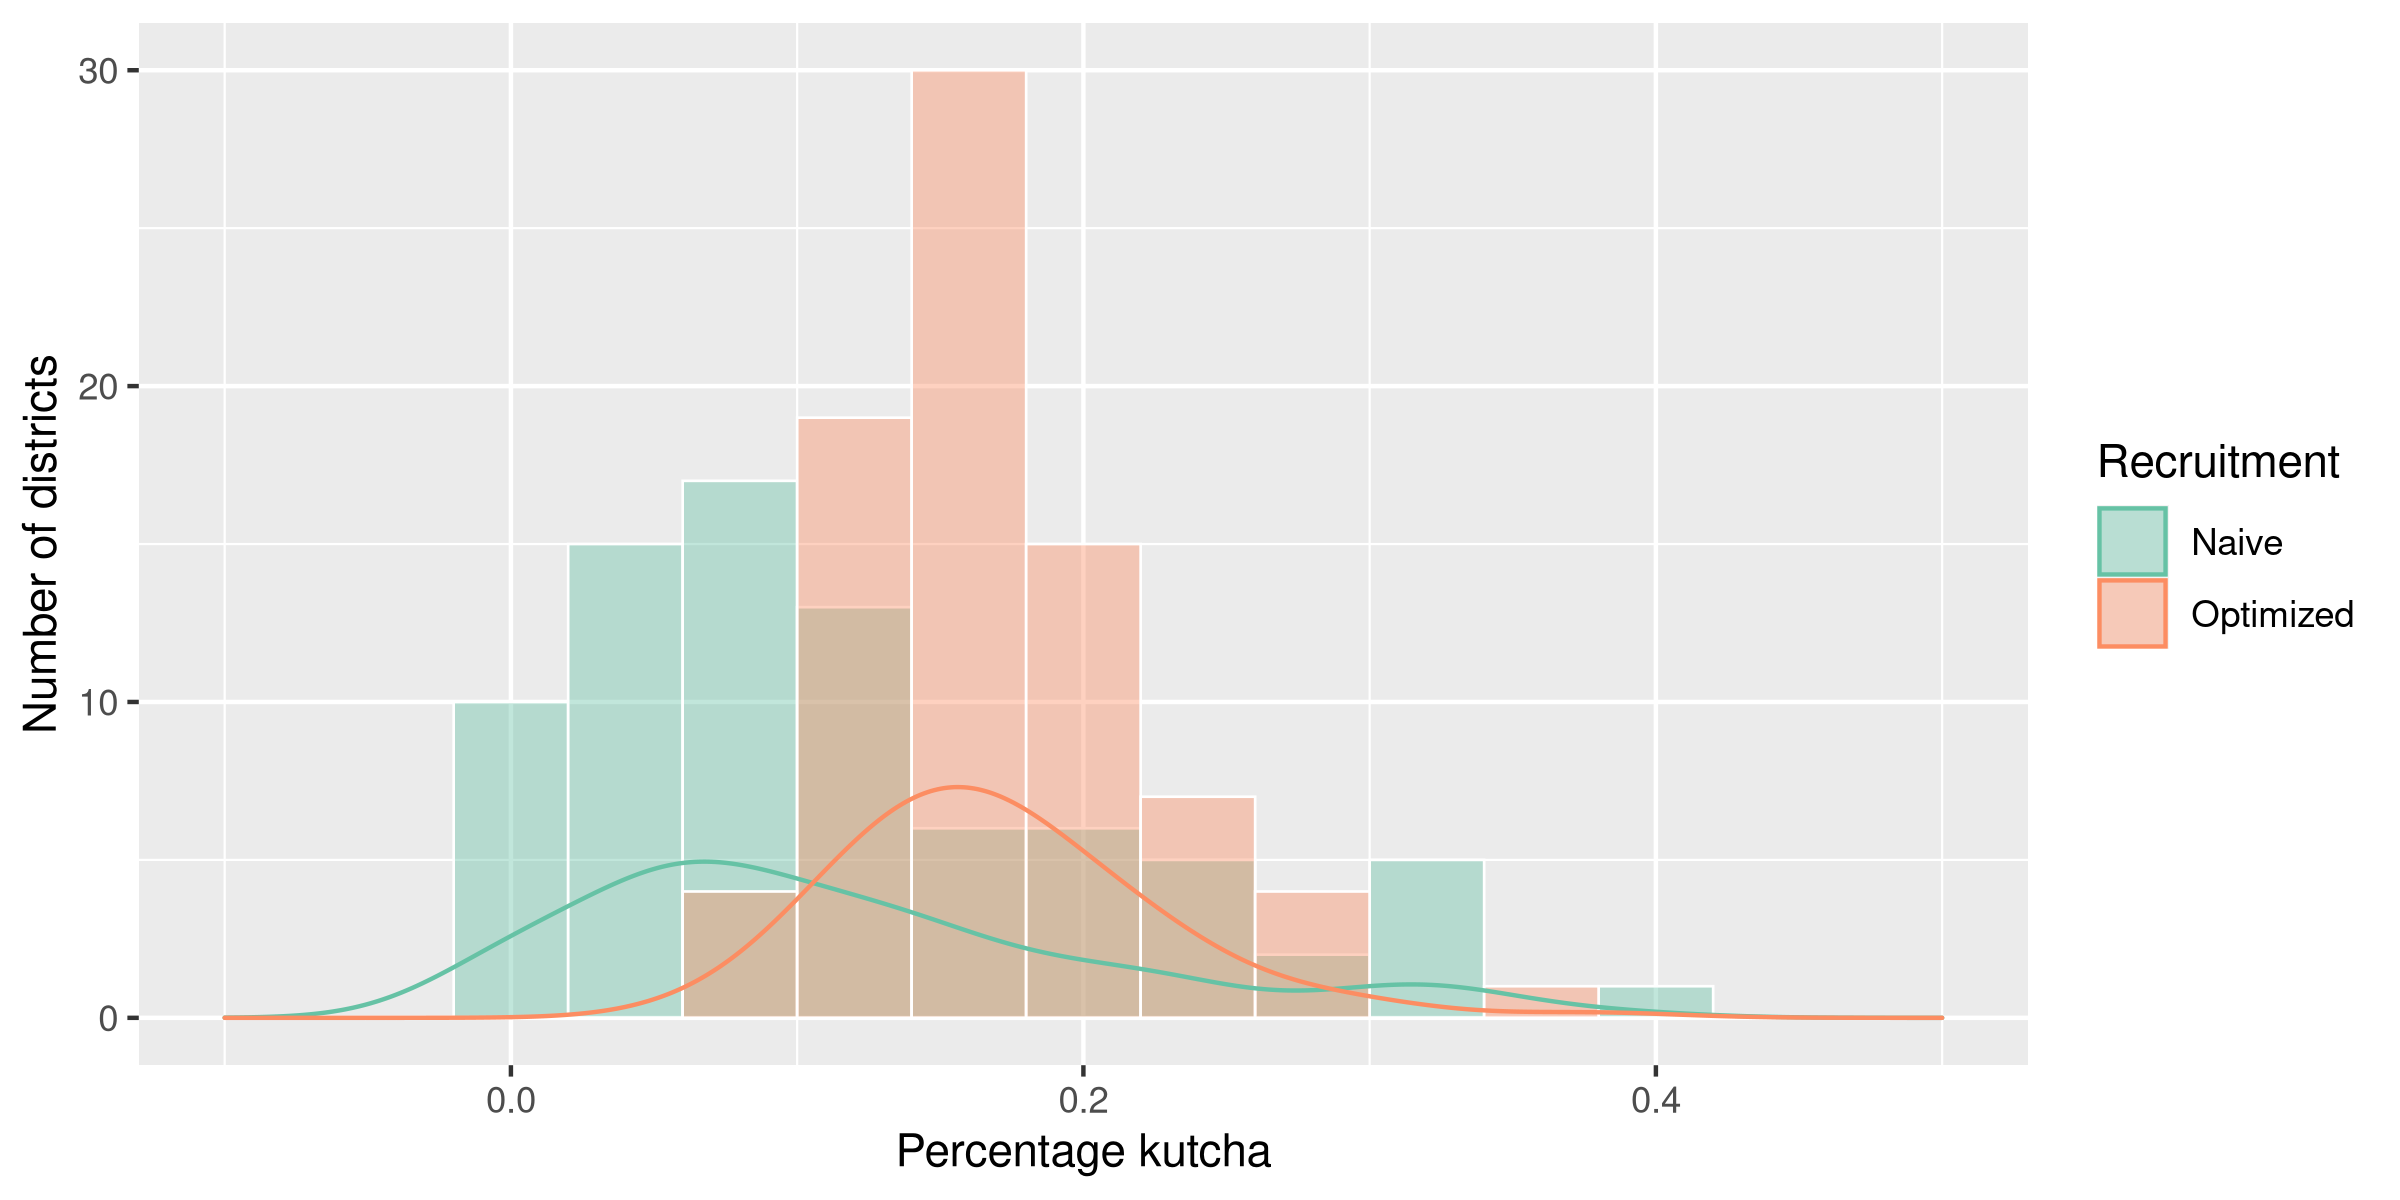
\includegraphics[width=\linewidth]{figures/recruitment}
	\caption{Recruitment}
    \label{fig:recruitment}
\end{figure}

\clearpage
\section{Additional Regression Tables}


% Table created by stargazer v.5.2.2 by Marek Hlavac, Harvard University. E-mail: hlavac at fas.harvard.edu
% Date and time: Sun, Jun 06, 2021 - 09:15:09 PM
\begin{table}[!htbp] \centering 
  \caption{Fever Incidence} 
  \label{tbl:Fever Incidence} 
\begin{tabular}{@{\extracolsep{5pt}}lcccccc} 
\\[-1.8ex]\hline 
\hline \\[-1.8ex] 
 & \multicolumn{3}{c}{Round 1 Panel} & \multicolumn{3}{c}{Round 2 Cross Section} \\ 
\\[-1.8ex] & (1) & (2) & (3) & (4) & (5) & (6)\\ 
\hline \\[-1.8ex] 
 treatment & $-$0.01 & 0.06 & $-$0.09 & $-$0.02 & $-$0.10 & 0.04 \\ 
  & (0.11) & (0.13) & (0.13) & (0.09) & (0.11) & (0.14) \\ 
  & & & & & & \\ 
 pucca &  & $-$0.22 &  &  & $-$0.03 &  \\ 
  &  & (0.15) &  &  & (0.11) &  \\ 
  & & & & & & \\ 
 semipucca &  & $-$0.07 &  &  & $-$0.05 &  \\ 
  &  & (0.13) &  &  & (0.09) &  \\ 
  & & & & & & \\ 
 treatment:pucca &  & $-$0.13 &  &  & 0.14 &  \\ 
  &  & (0.18) &  &  & (0.13) &  \\ 
  & & & & & & \\ 
\hline \\[-1.8ex] 
Controls & No & Yes & No & No & Yes & No \\ 
Subgroup & All & All & Pucca & All & All & Pucca \\ 
Observations & 3,508 & 3,508 & 1,741 & 4,899 & 4,896 & 2,192 \\ 
\hline 
\hline \\[-1.8ex] 
\textit{Note:}  & \multicolumn{6}{r}{$^{*}$p$<$0.1; $^{**}$p$<$0.05; $^{***}$p$<$0.01} \\ 
\end{tabular} 
\end{table} 



% Table created by stargazer v.5.2.2 by Marek Hlavac, Harvard University. E-mail: hlavac at fas.harvard.edu
% Date and time: Sun, Jun 06, 2021 - 09:15:08 PM
\begin{table}[!htbp] \centering 
  \caption{Malaria Incidence - OLS} 
  \label{tbl:Malaria Incidence - OLS} 
\begin{tabular}{@{\extracolsep{5pt}}lcccccc} 
\\[-1.8ex]\hline 
\hline \\[-1.8ex] 
 & \multicolumn{3}{c}{Round 1 Panel} & \multicolumn{3}{c}{Round 2 Cross Section} \\ 
\\[-1.8ex] & (1) & (2) & (3) & (4) & (5) & (6)\\ 
\hline \\[-1.8ex] 
 treatment & $-$0.01 & $-$0.02 & 0.01 & 0.01 & 0.02 & $-$0.01 \\ 
  & (0.01) & (0.01) & (0.01) & (0.01) & (0.01) & (0.01) \\ 
  & & & & & & \\ 
 pucca &  & $-$0.04$^{**}$ &  &  & $-$0.01 &  \\ 
  &  & (0.02) &  &  & (0.01) &  \\ 
  & & & & & & \\ 
 semipucca &  & $-$0.01 &  &  & $-$0.01 &  \\ 
  &  & (0.01) &  &  & (0.01) &  \\ 
  & & & & & & \\ 
 treatment:pucca &  & 0.03 &  &  & $-$0.03$^{**}$ &  \\ 
  &  & (0.02) &  &  & (0.01) &  \\ 
  & & & & & & \\ 
\hline \\[-1.8ex] 
Controls & No & Yes & No & No & Yes & No \\ 
Subgroup & All & All & Pucca & All & All & Pucca \\ 
Observations & 3,490 & 3,490 & 1,733 & 4,898 & 4,895 & 2,191 \\ 
\hline 
\hline \\[-1.8ex] 
\textit{Note:}  & \multicolumn{6}{r}{$^{*}$p$<$0.1; $^{**}$p$<$0.05; $^{***}$p$<$0.01} \\ 
\end{tabular} 
\end{table} 



% Table created by stargazer v.5.2.2 by Marek Hlavac, Harvard University. E-mail: hlavac at fas.harvard.edu
% Date and time: Sun, Jun 06, 2021 - 09:15:08 PM
\begin{table}[!htbp] \centering 
  \caption{Sleeping Under Bednet - OLS} 
  \label{tbl:Sleeping Under Bednet - OLS} 
\begin{tabular}{@{\extracolsep{5pt}}lcccccc} 
\\[-1.8ex]\hline 
\hline \\[-1.8ex] 
 & \multicolumn{3}{c}{Probability of Sleeping (Self)} & \multicolumn{3}{c}{Average Percentage of Household} \\ 
\\[-1.8ex] & (1) & (2) & (3) & (4) & (5) & (6)\\ 
\hline \\[-1.8ex] 
 treatment & 0.02 & $-$0.003 & 0.04 & 0.02 & $-$0.01 & 0.06$^{**}$ \\ 
  & (0.02) & (0.03) & (0.03) & (0.02) & (0.02) & (0.02) \\ 
  & & & & & & \\ 
 pucca &  & $-$0.06$^{**}$ &  &  & $-$0.09$^{***}$ &  \\ 
  &  & (0.03) &  &  & (0.02) &  \\ 
  & & & & & & \\ 
 semipucca &  & $-$0.02 &  &  & $-$0.03$^{*}$ &  \\ 
  &  & (0.02) &  &  & (0.02) &  \\ 
  & & & & & & \\ 
 treatment:pucca &  & 0.04 &  &  & 0.07$^{**}$ &  \\ 
  &  & (0.04) &  &  & (0.03) &  \\ 
  & & & & & & \\ 
\hline \\[-1.8ex] 
Controls & No & Yes & No & No & Yes & No \\ 
Subgroup & All & All & Pucca & All & All & Pucca \\ 
Observations & 2,972 & 2,972 & 1,415 & 2,697 & 2,697 & 1,311 \\ 
\hline 
\hline \\[-1.8ex] 
\textit{Note:}  & \multicolumn{6}{r}{$^{*}$p$<$0.1; $^{**}$p$<$0.05; $^{***}$p$<$0.01} \\ 
\end{tabular} 
\end{table} 



% Table created by stargazer v.5.2.2 by Marek Hlavac, Harvard University. E-mail: hlavac at fas.harvard.edu
% Date and time: Fri, Jun 04, 2021 - 11:26:42 PM
\begin{table}[!htbp] \centering 
  \caption{} 
  \label{tbl:Sleeping Under Bednet (Individual Level) - OLS} 
\small 
\begin{tabular}{@{\extracolsep{5pt}}lccccccc} 
\\[-1.8ex]\hline 
\hline \\[-1.8ex] 
 & \multicolumn{7}{c}{Sleeping Under Bednet (Individual Level) - OLS} \\ 
\cline{2-8} 
\\[-1.8ex] & \multicolumn{7}{c}{Slept Under Net} \\ 
\\[-1.8ex] & (1) & (2) & (3) & (4) & (5) & (6) & (7)\\ 
\hline \\[-1.8ex] 
 treatment & 0.01 &  & 0.02 & 0.03 & 0.02 & 0.02 & 0.02 \\ 
  & (0.04) &  & (0.03) & (0.04) & (0.03) & (0.03) & (0.03) \\ 
  & & & & & & & \\ 
 pucca & $-$0.13$^{***}$ &  & $-$0.11$^{***}$ &  & $-$0.14$^{***}$ & $-$0.12$^{***}$ &  \\ 
  & (0.04) &  & (0.04) &  & (0.04) & (0.05) &  \\ 
  & & & & & & & \\ 
 semipucca & $-$0.03 &  & $-$0.03 &  & $-$0.03 & $-$0.03 &  \\ 
  & (0.04) &  & (0.04) &  & (0.04) & (0.04) &  \\ 
  & & & & & & & \\ 
 ind\_treatment:pucca &  &  &  &  & 0.01 & 0.02 &  \\ 
  &  &  &  &  & (0.05) & (0.05) &  \\ 
  & & & & & & & \\ 
 admalaria &  &  &  &  &  &  & 0.12$^{***}$ \\ 
  &  &  &  &  &  &  & (0.03) \\ 
  & & & & & & & \\ 
 ind\_treatment & 0.07$^{***}$ & 0.06$^{**}$ & 0.07$^{***}$ & 0.07$^{**}$ & 0.06$^{*}$ & 0.06$^{*}$ & 0.06$^{**}$ \\ 
  & (0.03) & (0.03) & (0.03) & (0.04) & (0.04) & (0.04) & (0.03) \\ 
  & & & & & & & \\ 
 treatment:pucca & 0.03 &  &  &  &  &  &  \\ 
  & (0.05) &  &  &  &  &  &  \\ 
  & & & & & & & \\ 
 ind\_treatment:treatment &  &  &  & $-$0.02 &  &  &  \\ 
  &  &  &  & (0.05) &  &  &  \\ 
  & & & & & & & \\ 
 Constant & 0.75$^{***}$ & 0.69$^{***}$ & 0.75$^{***}$ & 0.69$^{***}$ & 0.75$^{***}$ & 0.75$^{***}$ & 0.68$^{***}$ \\ 
  & (0.04) & (0.02) & (0.04) & (0.03) & (0.04) & (0.04) & (0.03) \\ 
  & & & & & & & \\ 
\hline \\[-1.8ex] 
Controls & Yes & No & Yes & Yes & No & Yes & Yes \\ 
Observations & 1,225 & 1,226 & 1,225 & 1,225 & 1,226 & 1,225 & 1,225 \\ 
\hline 
\hline \\[-1.8ex] 
\textit{Note:}  & \multicolumn{7}{r}{$^{*}$p$<$0.1; $^{**}$p$<$0.05; $^{***}$p$<$0.01} \\ 
\end{tabular} 
\end{table} 









\end{document}